\documentclass[11pt]{article}

\usepackage{amsmath}
\usepackage{babel}
\usepackage[a4paper, margin={0.75in}]{geometry}
\usepackage{minted}
\usepackage{float}
\usepackage{multicol}
\usepackage{graphicx}

\begin{document}
    \begin{center}
        \LARGE{Odpowiedzi na pytania do egzaminu z APU} \\
        \Large{Wykłady 1--3}
    \end{center}

    \vspace{2cm}
    
    \section{Wykład}
    \begin{enumerate}
        \item Definicja procesów uczenia \\
        Nie ma jednej definicji procesów uczenia się:
        \begin{itemize}
            \item ``Uczenie się oznacza zmiany w systemie, które mają charakter adaptacyjny
            w tym sensie, że pozwalają systemowi wykonać za następnym razem takie
            same zadanie lub zadania podobne bardziej efektywnie'' - Herbert Simon
            (1983)
            \item ``System uczący się wykorzystuje zewnętrzne dane empiryczne w celu tworzenia
            i aktualizacji podstaw dla udoskonalania działania na podobnych danych w przyszłości
            oraz wyrażania tych podstaw w zrozumiałej i symbolicznej postaci'' - Donald Miche
            (1991)
            \item ``Uczenie sie to konstruowanie i zmiana reprezentacji doświadczanych
            faktów.
            W ocenie konstruowanych reprezentacji bierze się pod uwagę:
            \begin{enumerate}
                \item wiarygodność - określa stopień w jakim reprezentacja odpowiada rzeczywistości;
                \item efektywność - charakteryzuje przydatność reprezentacji do osiągania danego celu;
                \item poziom abstrakcji - odpowiada zakresowi szczegółowości i precyzji pojęć używanych
                w reprezentacji; określa on tzw.\ moc opisową reprezentacji.
                Reprezentacja jest rozumiana jako np.\ opisy symboliczne, algorytmy,
                modele symulacyjne, plany obrazy.'' - Ryszard Michalski (1986)
            \end{enumerate}
            \item Elementem wspólnym tych definicji są: Wejście (dane empiryczne), miara oceny (Zmiany 
            i poprawa działania) oraz postulat zdobywania wiedzy, reprezentowania jej wewnątrz systemu
            i stosowania jej do wykonania zadania (nacisk na zrozumiałość reprezentacji)
        \end{itemize}
        \item Przykłady problemów rozwiązywanych przez systemy uczące się \\
        \begin{itemize}
            \item Uczenie się rozpoznawania mowy
            \item Uczenie się kierowania pojazdem (np.\ ALVINN)
            \item Uczenie się klasyfikacji obiektów astronomicznych (NASA Sky Survey)
            \item Uczenie się rozgrywania pewnych gier
            \item Uczenie się rozpoznawania chorób na podstawie symptomów
            \item Uczenie się rozpoznawanie pisma na podstawie przykładów
            \item Uczenie się klasyfikowania tekstów do grup tematycznych
            \item Uczenie się aproksymacji nieznanej funkcji na podstawie próbek
            \item Uczenie się odnajdowania drogi w nieznanym środowisku
            \item Automatyczne odkrywanie zależności funkcyjnych w danych
            \item Przewidywanie trendów w danych finansowych
        \end{itemize}
        \clearpage
        \item Motywacje dla budowy systemów uczących się
        \begin{itemize}
            \item Zadania eksploracji i analizy danych, gdzie duże rozmiary zbiorów
            danych uniemożliwiają ich analizę w sposób nieautomatyczny (np.
            ekonomiczne lub medyczne bazy danych)
            \item Środowiska gdzie system musi się dynamicznie dostosowywać do
            zmieniających się warunków (np.\ systemy sterowania)
            \item Problemy które są złożone, trudne do opisu i często nie posiadają
            wystarczających modeli teoretycznych albo ich uzyskanie jest bardzo
            kosztowne lub mało wiarygodne.
        \end{itemize}
        \item Klasyfikacja metod maszynowego uczenia się
        \begin{itemize}
            \item Uczenie indukcyjne - na podstawie znanych faktów i obserwacji tworzona
            jest uogólnienie, które próbuje dopasować wszystkie znane fakty do hipotezy
            \item ``Nabywanie umiejętności'' - optymalizacja zastosowania już posiadanej
            wiedzy w sposób zwiększający jej efektywność
        \end{itemize}
        \item Tworzenie modelu uczenia maszynowego
        \begin{enumerate}
            \item Przygotowanie danych (zebranie danych, uzupełnienie braków, normalizacja)
            \item Zdefiniowanie zadania (regresja, klasyfikacja, grupowanie, inne)
            \item Wybór metody (regresja liniowa, logistyczna, drzewa decyzyjne,
            sieci neuronowe)
            \item Strojenie parametrów
            \item Ocena modelu
        \end{enumerate}
        \item Język R. Wykonywanie instrukcji\\
        Sekwencyjne, możliwe wpisywanie kolejnych poleceń z konsoli lub z pliku skryptu
        o rozszerzeniu *.R.
        W konsoli występuje znak zachęty \mintinline{text}|>|.
        Komentarz tworzony jest przez \mintinline{r}|#|.
        Zapisywanie ma postać \mintinline{r}|zmienna <- wartość|.
        \item Korzystanie z pomocy R
        \begin{itemize}
        	\item \mintinline{r}|help(max)| - klasyczna pomoc
        	\item \mintinline{r}|?max| - skrócona wersja
        	\item \mintinline{r}|example(max)| - przykłady użycia
        	\item \mintinline{r}|RSiteSearch("max function")| - przeszukiwanie forum
        	\item \mintinline{r}|apropos("max", mode = "function")| - wyszukiwanie z funkcji z nazwą "max"
        	\item \mintinline{r}|data()| - nazwy obiektów w pakiecie
        	\item \mintinline{r}|vignette()| - pdf z dokumentacją
        \end{itemize}
        \item Zarządzanie obszarem roboczym R
        \begin{itemize}
        	\item \mintinline{r}|getwd()| - ścieżka do aktualnego katalogu roboczego
        	\item \mintinline{r}|setwd("..")| - ustawia nową ścieżkę do katalogu roboczego
        	\item \mintinline{r}|ls()| - wyświetla zmienne obszaru roboczego
        	\item \mintinline{r}|remove(a, b, c)| - usuwa zmienne a, b, c z obszaru roboczego
        	\item \mintinline{r}|history(3)| - 3 ostatnio użyte instrukcje
        	\item \mintinline{r}|savehistory("plik.txt")| - zapisuje historię do pliku
        	\item \mintinline{r}|loadhistory("plik.txt")| - odczyt historii z pliku
        	\item \mintinline{r}|save.image("workspace.RData")| - zapis obszaru roboczego do pliku
        	\item \mintinline{r}|save(a, b, c, file = "workspace.RData")| - zapis tylko kilku zmiennych do pliku
        	\item \mintinline{r}|load("workspace.RData")| - odczyt obszaru roboczego z pliku
        \end{itemize}
        \item Pakiety rozszerzające R
        \begin{itemize}
        	\item \mintinline{r}|installed.packages()| - lista zainstalowanych paczek
        	\item \mintinline{r}|search()| - wyszukiwanie w załadowanych paczkach
        	\item \mintinline{r}|install.packages("RWeka")| - instalowanie paczki RWeka
        	\item \mintinline{r}|library(RWeka)| - ładowanie paczki RWeka
        \end{itemize}
        \item Skalary i wektory R \\
        Skalary obejmują pojedyncze liczby, łańcuchy znaków i wartości logiczne.
        Typ każdej zmiennej i wyrażenia można sprawdzić funkcją \mintinline{r}|class(obj)|.
        Np. \mintinline{r}|class(2)| zwróci \mintinline{text}|[1] "numeric"|.
        Każda liczba (bez względu czy double czy int) to numeric. \\
        Operacje na liczbach:
        \begin{itemize}
        	\item +, -, *, / (dodawanie, odejmowanie, mnożenie, dzielenie)
        	\item \%\% (modulo)
        	\item \^ (potęga)
        	\item sqrt(n) (pierwiastek kwadratowy)
        \end{itemize}
        Dla znaków łączenie nie działa z + tylko z funkcją \mintinline{r}|paste("a", "b", "c", sep=" ")|.
        Dla typów logicznych operacje porównania są takie same jak w C++ czy Csharp. \\
        Wektor obejmuje wiele skalarów tego samego typu.
        Są jednowymiarowe.
        Do utworzenia wektora używa się funkcji \mintinline{r}|c(obj, ...)|.
        Próba utworzenia wektora o różnych typach spowoduje konwersję typów. \\
        Można utworzyć sekwencję, która będzie również zachowywała się jak wektor.
        Tworzy się ją przy użyciu operatora \mintinline{r}|<liczba>:<liczba>| lub funkcji \mintinline{r}|seq(<liczba>, <liczba>, <krok>)|.
        Wektory indeksujemy od 1, a nie od 0.
        Ujemne wartości w indeksie to pobranie wszystkiego \textbf{oprócz} ostatnich N.
        W indekserze można użyć wektora indeksów.
        Zwróci on wtedy wektor z wartościami o indeksach jakie zostały wskazane.
        Można też użyć sekwencji do pobierania tych wartości. \\
        Do sprawdzenia długości wektora używa się \mintinline{r}|length(vect)|.
        \item Ramka danych R \\
        Ramka danych to powiązanie dwóch wektorów o tej samej długości. Np. imię i wiek.
        Do jej utworzenia używa się \mintinline{r}|data.frame(label = vector, label = vector)|.
        \mintinline{r}|names(ramka)| pozwala na wyświetlenie nazw kolumn.
        Konstrukcja \mintinline{r}|names(ramka) <- c ("abc", "cde")| umożliwia nadpisanie nazw w ramce.
        Indeksując ramkę indeksujemy wiersze, ale możemy użyć konstrukcji \mintinline{r}|frame[1, 1]| co zwróci nam dane tylko z pierwszej kolumny.
        Korzystając z operatora \mintinline{r}|ramka$abc| można pobrać kolumnę po nazwie.
        Można indeksować podając warunek: \mintinline{r}|ramka[ramka$abc < 10]|. \\
        Dodawanie nowego wiersza możliwe jest przy użyciu funkcji \mintinline{r}|rbind(old, new)|.
        Odpowiednio dodawanie kolumny wymaga funkcji \mintinline{r}|cbind(old, new)|. \\
        Dodatkowe funkcje które pozwalają uzyskać informacje o ramce:
        \begin{itemize}
        	\item \mintinline{r}|lenght(ramka)| - Liczba kolumn w ramce
        	\item \mintinline{r}|dim(ramka)| - Wymiary ramki
        	\item \mintinline{r}|str(ramka)| - Tekstowy opis zawartości ramki
        	\item \mintinline{r}|head(ramka, n = 2)| - Wyświetlenie pierwszych 2 wierszy w ramce
        	\item \mintinline{r}|tail(ramka, n = 2)| - Wyświetlenie ostatnich 2 wierszy w ramce
        \end{itemize}
        \clearpage
        \item Przegląd wykresów
        \begin{itemize}
        	\item Histogram 
        	\begin{minted}{r}
hist(vector,
	breaks = unique(vector),
	right = FALSE, 
	main = "Main title", 
	xlab = "Label x", 
	ylab = "Label y")
        	\end{minted}
        	
        	\item Wykres pudełkowy - wizualizuje minimum, pierwszy kwartyl (0.25), medianę, drugi kwartyl (0.25) i wartość maksymalną
        	\begin{minted}{r}
boxplot(iris$Sepal.Width,
	main = "Podstawowe staystyki dla szerokosci kwiatu sepal")
        	\end{minted}
        	
        	\item Wykres kołowy
        	\begin{minted}{r}
pie(table(new_iris$Species) / length(new_iris$Species))
        	\end{minted}
        	
        	\item Wykres wachlarzowy
        	\begin{minted}{r}
install.packages("plotrix")
library(plotrix)
fan.plot(percentage, labels = names(percentage))
        	\end{minted}
        	
        	\item Wykres słupkowy
        	\begin{minted}{r}
count <- table(new_iris$Species)
colors <- rainbow(3)
barplot(count,
	main = "Liczebnosc gatunkow",
	ylim = c(0, 50),
	xlab = "Gatunek",
	ylab = "Ilosc",
	col = colors)
        	\end{minted}
        	
        	\begin{figure}[H]
        		\begin{minipage}{.5\textwidth}
        			\centering
        			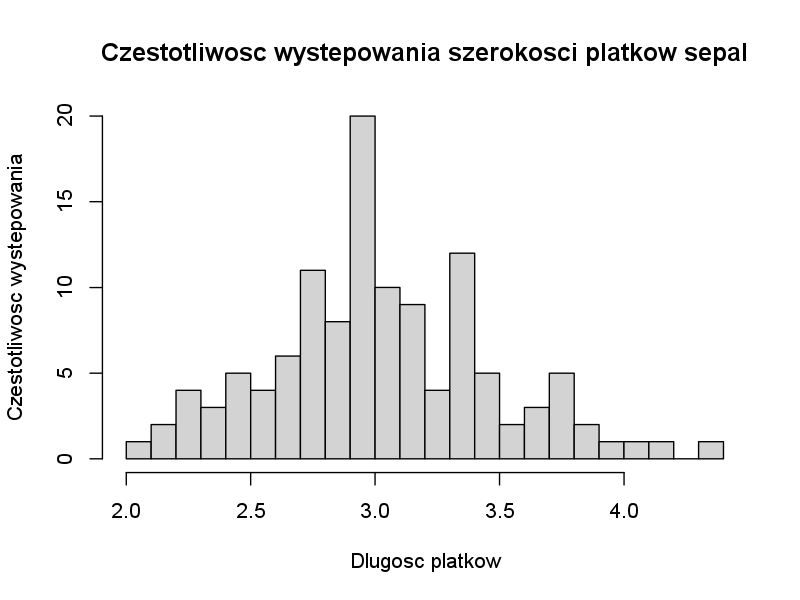
\includegraphics[width=\textwidth]{imgs/hist}
        			\caption{Histogram}
        		\end{minipage}
        		\begin{minipage}{.5\textwidth}
        			\centering
        			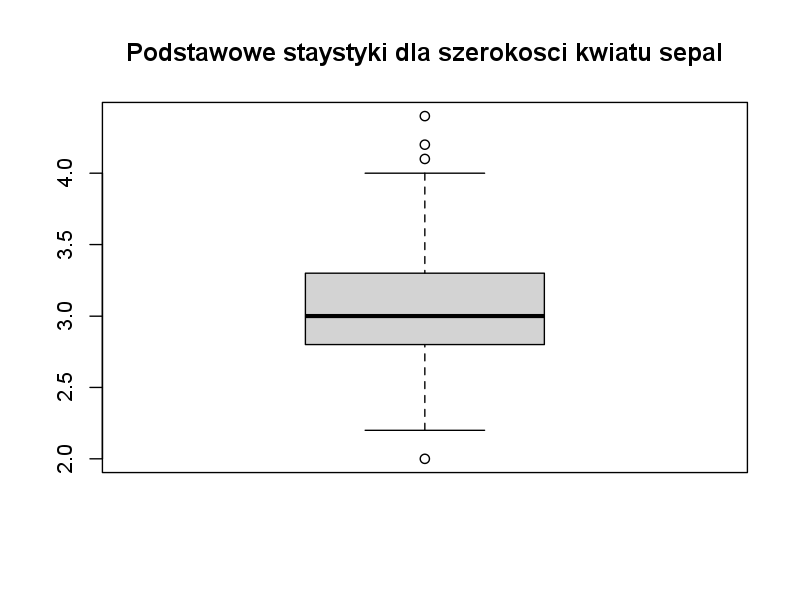
\includegraphics[width=\textwidth]{imgs/box}
        			\caption{Wykres pudełkowy}
        		\end{minipage}
        	\end{figure}
        	\begin{figure}[H]
        		\begin{minipage}{.5\textwidth}
        			\centering
        			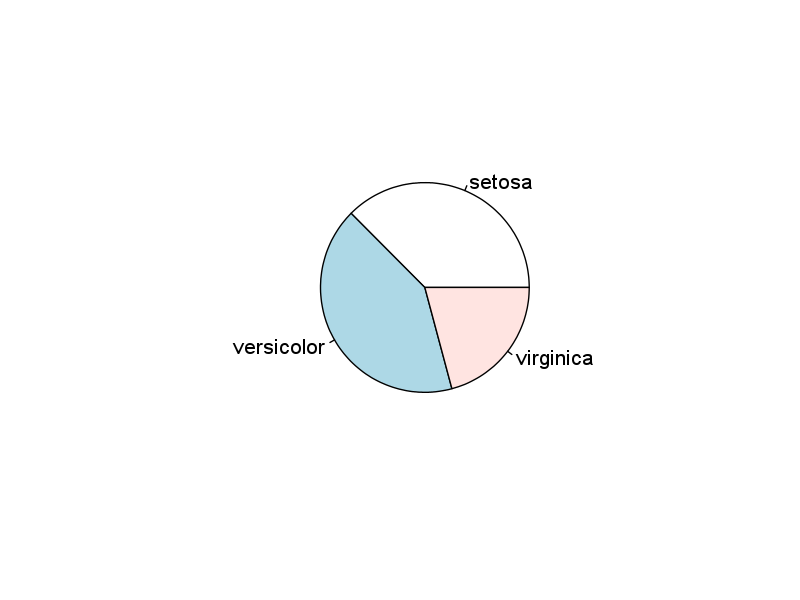
\includegraphics[width=\textwidth]{imgs/pie}
        			\caption{Wykres kołowy}
        		\end{minipage}
        		\begin{minipage}{.5\textwidth}
        			\centering
        			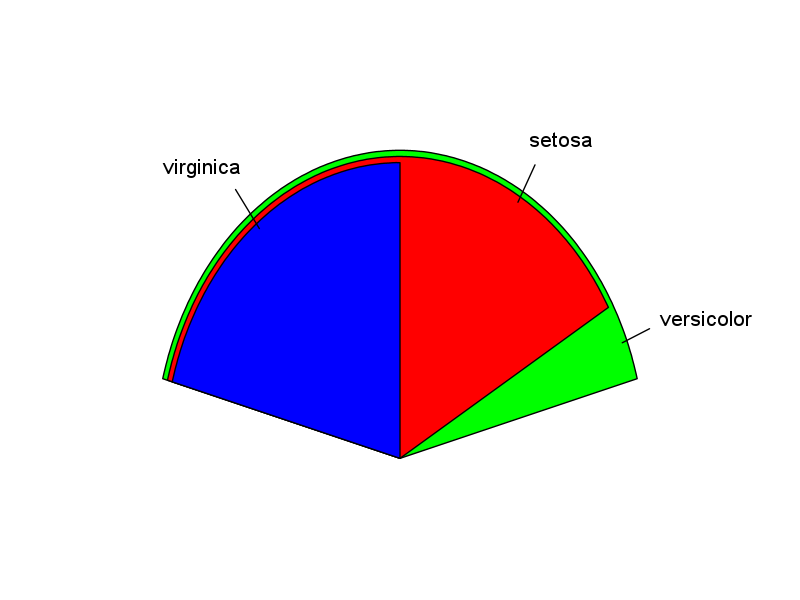
\includegraphics[width=\textwidth]{imgs/fan}
        			\caption{Wykres wachlarzowy}
        		\end{minipage}
        	\end{figure}
        	\begin{figure}[H]
        		\centering
        		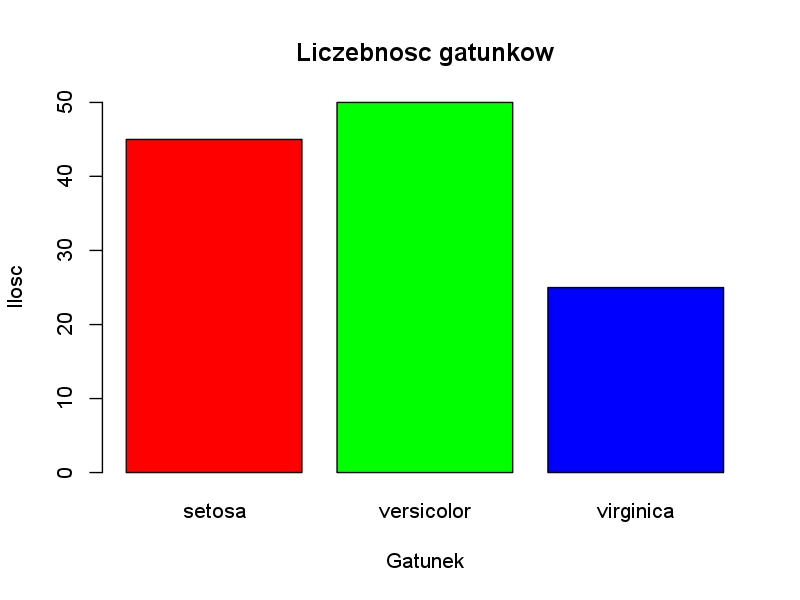
\includegraphics[width=.5\textwidth]{imgs/barplot}
        		\caption{Wykres słupkowy}
        	\end{figure}
        \end{itemize}
        \item Język R i uczenie maszynowe
        \begin{itemize}
        	\item Składniki uczenia maszynowego - szereg konceptów uczenia maszynowego
        	\item Zbiór uczący - doświadczenie w postaci danych. 
        	Zbiór może być etykietowany lub nieetykietowany.
        	\item Atrybuty (cechy) - opis obiektów zbioru uczącego
        	\item Instancja - zestaw atrybutów opisujących jeden obiekt
        	\item Model - utworzone na podstawie danych rozwiązanie zadania
        	\begin{itemize}
        		\item Geometryczny - oparty o przestrzeń euklidesową.
        		Tworzony przez regresję liniową, logistyczną lub maszynę wektorów
        		wspierających (SVM, SMO)
        		\item Logiczny - oparty o logiki matematyczne. Zawiera proste reguły
        		w postaci warunków prowadzących do decyzji. Tworzony przez drzewa
        		decyzyjne, JRipper, PART
        		\item Probabilistyczny - oparty o prawdopodobieństwo warunkowe
        		i regułę Bayesa
        		\item Hybrydowe
        	\end{itemize}
        	\item Ewaluacja - sposoby oceny skuteczności modelu
        	\begin{itemize}
        		\item Podział na zbiory uczący i testowy
        		\item 10-fold cross-validation - 10-krotne powtórzenie podziału zbioru
        		uczącego. Efekt końcowy jest uśrednieniem poprzednich pomiarów.
        	\end{itemize}
        \end{itemize}
    \end{enumerate}
    \section{Wykład}
    \begin{enumerate}
        \item Analiza eksploracyjna i analiza potwierdzająca \\
        Analiza potwierdzająca polega na odrzuceniu fałszywych wzorców.
        Do tego używa się najczęściej metod:
        \begin{itemize}
        	\item testowania formalnego - sprawdzenie zachowania modelu przy użyciu
        	danych nie użytych w analizie eksploracyjnej;
        	\item teorii prawdopodobieństwa - sprawdzenie czy wzorce w pierwotnej próbce
        	mogły powstać przypadkowo.
        \end{itemize}
        Analiza eksploracyjna to stosowanie różnych technik prowadzących do wykrycia
        zależności między danymi i powstania modeli. Ludzie mają tendencję do
        znajdowania fałszywych wzorców, które nie istnieją. Analiza eksploracyjna
        musi być uzupełniona analizą potwierdzającą.
        
        \item Czym są dane w uczeniu maszynowym?
        Zbiór danych to tabela w której wiersze odpowiadają za obserwacje zjawisk,
        a kolumny opisują cechy (atrybuty) tej obserwacji. Dane układające się
        w formie tabeli nazywa się modelem danych prostokątnych. \\
        Operacje na takich danych można wizualizować rysunkami. Innym sposobem
        na uproszczenie zbioru jest podsumowanie liczbowe.
        
        \item Wnioskowanie o typach danych w kolumnach
        \begin{itemize}
        	\item \mintinline{r}|is.numeric(obj)|
        	\item \mintinline{r}|is.character(obj)|
        	\item \mintinline{r}|is.factor(obj)| - sprawdza czy wartości są skategoryzowane (zmienne typu factor). Zmienna taka wewnętrznie jest liczbą,
        	ale gdy jest wyświetlana to tłumaczona zostaje na ciąg znaków.
        \end{itemize}
        
        \item Podsumowania liczbowe w R \\
        \mintinline{r}|summary(ramka)| - tworzy zestawienie składające się z minimum,
        kwantyla pierwszego, mediany, średniej, kwantyla trzeciego i wartości maksymalnej.
        
        \item Średnie, mediany i dominanty w R
        \begin{itemize}
        	\item \mintinline{r}|mean(obj)| - średnia
        	\item \mintinline{r}|median(obj)| - mediana
        	\item dominanty nie da się wyznaczyć wbudowaną funkcją ze względu na
        	brak możliwości porównywania liczb zmiennoprzecinkowych, co jest 
        	wymagane definicją.
        \end{itemize}
        
        \item Kwantyle w R
        \begin{itemize}
        	\item \mintinline{r}|quantile(vec)| - zwraca wartości dla 0, 25\%, 50\%,
        	75\% i 100\%.
        	\item \mintinline{r}|quantile(vec, probs=seq(0, 1, by=0.20))| - zwraca wartości dla co 20\% od 0 do 100\%.
        \end{itemize}
        
        \item Odchylenia standardowe i wariancje w R
        \begin{itemize}
        	\item \mintinline{r}|var(vec)| - wariancja
        	\item \mintinline{r}|sd(vec)| - odchylenie standardowe
        \end{itemize}
        
        \clearpage
        \item Eksploracyjne wizualizacje danych
        Do użycia funkcji \mintinline{r}|ggplot| potrzeba załadować bibliotekę
        \begin{itemize}
        	\item Histogram
        	\begin{minted}{r}
ggplot(iris, aes(x = Sepal.Length)) + 
geom_histogram(binwidth = 0.1) + 
labs(x = "Sepal.Length", y = "liczba")
        	\end{minted}
        	\item Wykres gęstości (ang. \textit{kernel density estimates} - KDE)
        	\begin{minted}{r}
ggplot(iris, aes(x = Sepal.Length)) + 
geom_density() + 
labs(x = "Sepal.Length", y = "liczba")
        	\end{minted}
        \end{itemize}
        \begin{figure}[H]
        	\begin{minipage}{.5\textwidth}
        		\centering
        		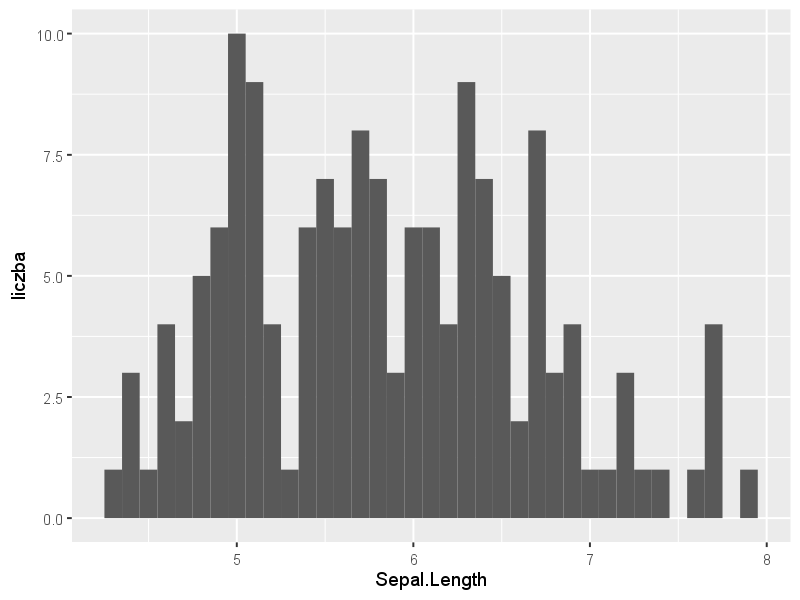
\includegraphics[width=\textwidth]{imgs/ggplot_hist}
        		\caption{Histogram z ggplot}
        	\end{minipage}
        	\begin{minipage}{.5\textwidth}
        		\centering
        		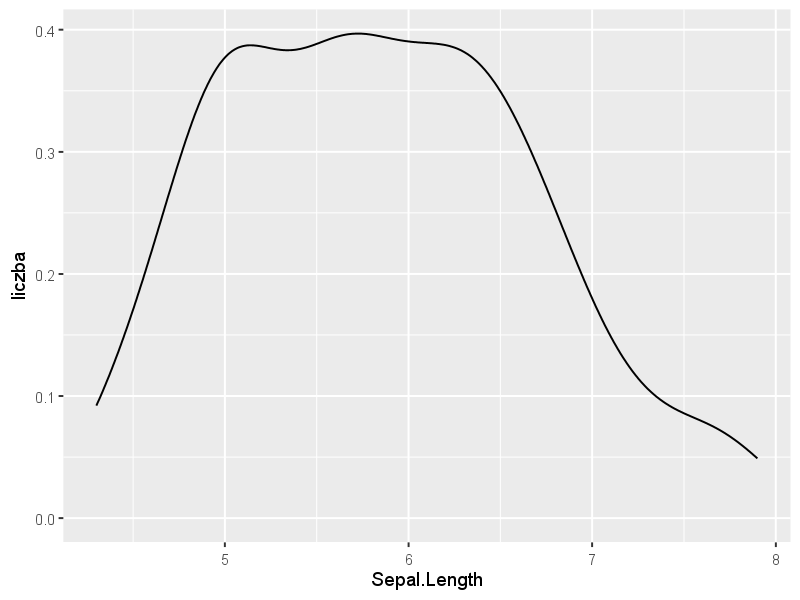
\includegraphics[width=\textwidth]{imgs/ggplot_dense}
        		\caption{Wykres gęstości}
        	\end{minipage}
        \end{figure}
        Generowanie rozkładów:
        \begin{itemize}
        	\item Normalny - \mintinline{r}|rnorm(próbki, ymin, ymax)|
        	\item Cauchy - \mintinline{r}|rcauchy(próbki, ymin, ymax)|
        	\item Gamma - \mintinline{r}|rgamma(próbki, ymin, ymax)|
        	\item Wykładniczy - \mintinline{r}|rexp(próbki, ymin, ymax)|
        \end{itemize}
        
        \clearpage
        \item Wizualizowanie powiązań pomiędzy kolumnami
        Wykresy przedstawiające powiązania między atrybutami:
        \begin{itemize}
        	\item Wykres punktowy
        	\begin{minted}{r}
ggplot(iris, aes(x = Sepal.Length, y = Petal.Length, color = Species)) + 
geom_point() + 
labs(x = "Sepal.Length", y = "Petal.Length", color = "Species")
        	\end{minted}
        	\item Wygładzony wykres punktowy
        	\begin{minted}{r}
ggplot(iris, aes(x = Sepal.Length, y = Petal.Length, color = Species)) + 
geom_point() + 
labs(x = "Sepal.Length", y = "Petal.Length", color = "Species") + 
geom_smooth()
        	\end{minted}
        \end{itemize}
        \begin{figure}[H]
        	\begin{minipage}{.5\textwidth}
        		\centering
        		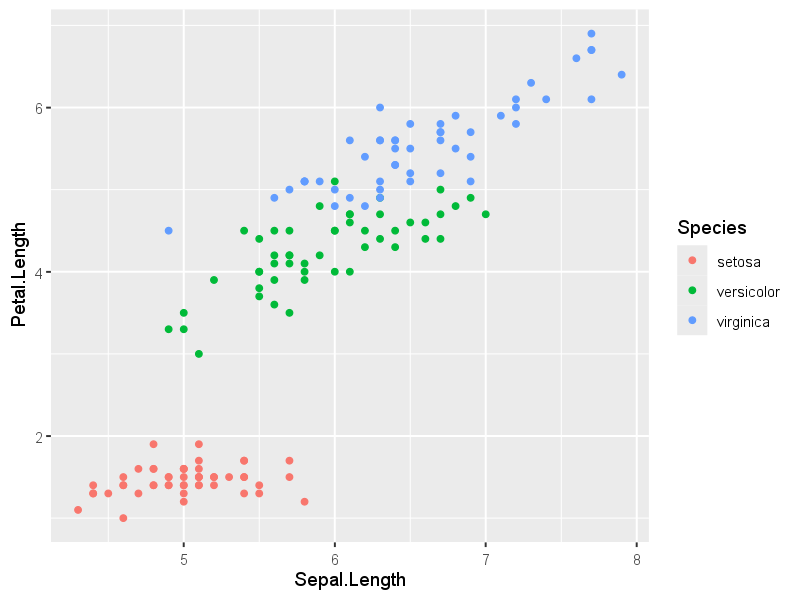
\includegraphics[width=\textwidth]{imgs/ggplot_point}
        		\caption{Wykres punktowy}
        	\end{minipage}
        	\begin{minipage}{.5\textwidth}
        		\centering
        		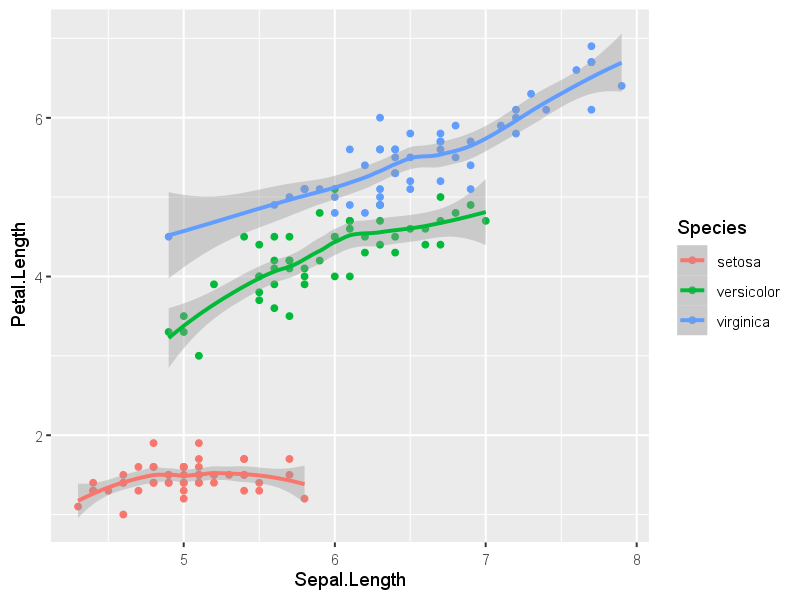
\includegraphics[width=\textwidth]{imgs/ggplot_smooth}
        		\caption{Wykres punktowy wygładzony}
        	\end{minipage}
        \end{figure}
        % wykład 4 - piątek
        \item Klasyfikacja; Zdefiniowanie zadania
        \item Trening i testowanie klasyfikacji
        \item Kryteria porównawcze metod klasyfikacji
        \item Metody klasyfikacji
        \item Drzewa decyzyjne
        \item Funkcje testu w celu konstruowania drzew decyzyjnych
        \item Konstrukcja drzew decyzyjnych
        \item Problem brakujących wartości przy konstruowaniu drzew decyzyjnych
        \item Analiza ROC jakości klasyfikacji
        \item Krzywe ROC
        \item Czułość, a specyficzność klasyfikacji binarnej
        \item Konstruowanie krzywych ROC
        \item Pakiet ROCR
    \end{enumerate}
    
    \section{Wykład}
    \begin{enumerate}
        \item Wieloatrybutowe problemy decyzyjne
        \item Proces analitycznej hierarchizacji problemu decyzyjnego
        \item Kroki rozwiązywania problemu AHP
        \item Podstawy wieloatrybutowej teorii użyteczności
        \item Agregacja ocen z wykorzystaniem macierzy porównań parami
        \item Skala preferencji względnej
        \item Ocena spójności macierzy porównań parami
        \item Krok V – obliczenie priorytetów AHP
        \item Obliczanie przybliżonego wektora własnego macierzy porównań parami
        \item Inne metody rozwiązywania problemu AHP
        \item Przykłady zastosowań metody AHP
    \end{enumerate}
\end{document}